\documentclass[11pt]{article}

% Standard packages
\usepackage[utf8]{inputenc}
\usepackage[T1]{fontenc}
\usepackage{amsmath,amssymb,amsfonts,amsthm}
\usepackage{algorithmic}
\usepackage{algorithm}
\usepackage{graphicx}
\usepackage{textcomp}
\usepackage{xcolor}
\usepackage{booktabs}
\usepackage{hyperref}
\usepackage{multirow}
\usepackage{geometry}
\usepackage{enumitem}
\usepackage{natbib}
\usepackage{tikz}
\usetikzlibrary{shapes,arrows.meta,positioning,fit,calc,decorations.pathreplacing}

\geometry{margin=1in}

% Theorem environments
\newtheorem{definition}{Definition}
\newtheorem{proposition}{Proposition}
\newtheorem{theorem}{Theorem}

% Custom commands
\newcommand{\efa}{\textsc{EFA}}  % Evaluation-First Architecture
\newcommand{\cmpg}{\textsc{CMPG}}
\newcommand{\fwrl}{\textsc{FWRL}}
\newcommand{\R}{\mathbb{R}}
\newcommand{\E}{\mathbb{E}}
\newcommand{\calC}{\mathcal{C}}
\newcommand{\calG}{\mathcal{G}}
\newcommand{\calE}{\mathcal{E}}
\newcommand{\calD}{\mathcal{D}} % Criteria space (distinct from generator \calC)

\title{\textbf{Evaluation-First Generation: Specification-Driven LLM Output Quality \\ via Dynamic Rubric Conditioning and Iterative Criteria Refinement}}

\author{
Karthick Raja M \\
Independent Researcher \\
Chennai, India \\
\texttt{karthickrajam18@gmail.com}
}

\date{March 2026}

\begin{document}

\maketitle

% ============================================================================
% ABSTRACT
% ============================================================================
\begin{abstract}
Current large language model (LLM) generation pipelines treat evaluation as a post-hoc measurement step: generate first, evaluate later. This separation means models generate ``blindly'' without explicit awareness of the quality dimensions they must satisfy, and refinement feedback---when provided---is holistic rather than dimension-specific. We propose \textbf{Evaluation-First Architecture} (\efa{}), a prompt-level generation framework that inverts this paradigm by generating query-specific evaluation criteria \emph{before} generation and using them as structured conditioning targets throughout the generation process. \efa{} introduces two novel mechanisms: (1) \textbf{Criteria-Masked Progressive Generation} (\cmpg{}), which progressively unmasks quality dimensions during generation analogous to causal token masking but over evaluation criteria, and (2) \textbf{Failure-Weighted Reattention Loop} (\fwrl{}), which maps per-criterion evaluation scores to criterion emphasis adjustments, amplifying focus on failing dimensions in subsequent generation passes. We formalize the framework, analyze convergence properties under monotonic improvement assumptions, and evaluate on 80 MT-Bench prompts using cross-model evaluation (MiniMax-M2.5 generator, Ollama Qwen-3.5-9B evaluator) to eliminate self-preference bias. \efa{} achieves 96.2\% All-Pass Rate (APR), outperforming all seven baselines including single-pass generation (71.2\%), Self-Refine (92.5\%), Best-of-5 (91.2\%), and FusioN (92.5\%). Ablation studies confirm that iterative refinement ($-12.4$pp) and dynamic criteria generation ($-7.4$pp) are the primary contributors, while \cmpg{} provides a meaningful $+3.7$pp gain. We present an honest analysis showing that \fwrl{}'s failure-proportional reweighting yields no measurable improvement over uniform reweighting on this benchmark---an ablation variant without \fwrl{} matches \efa{}'s APR and achieves slightly higher RAS---likely due to a ceiling effect with strong generators. To our knowledge, no prior work in the general text generation domain uses dynamically-generated evaluation rubrics as inference-time generation specifications with failure-proportional reweighting.
\end{abstract}

% ============================================================================
% 1. INTRODUCTION
% ============================================================================
\section{Introduction}

The dominant paradigm for improving LLM output quality follows a \emph{generate-then-evaluate} pattern: a model produces an output, a separate evaluation step scores it, and---optionally---the model refines based on feedback \citep{madaan2023selfrefine, shinn2023reflexion, gou2024critic}. While effective, this paradigm suffers from three fundamental limitations.

First, \textbf{evaluation is disconnected from generation}. The model has no explicit awareness of what quality dimensions it must satisfy during the generation process itself. Rubric-based reward models \citep{li2025openrubrics, zhang2025carmo} generate sophisticated per-query evaluation criteria but use them exclusively for post-hoc scoring, never as generation targets. This is analogous to writing code without knowing the test suite---possible, but needlessly inefficient.

Second, \textbf{refinement feedback is holistic, not dimensional}. Self-Refine \citep{madaan2023selfrefine} produces textual feedback like ``the response lacks specificity,'' requiring the model to implicitly parse which quality dimensions failed. The self-refinement literature itself identifies this as the core bottleneck: diagnosis---not repair---is the primary challenge \citep{lee2025refinebench}. Models achieve near-perfect refinement when given targeted, structured feedback but struggle with self-diagnosis.

Third, \textbf{all quality dimensions receive equal emphasis}. Whether a response perfectly satisfies relevance but catastrophically fails on factual accuracy, subsequent refinement passes treat all dimensions uniformly. No existing system allocates more generation ``budget'' to failing dimensions.

We propose \textbf{Evaluation-First Architecture} (\efa{}), a prompt-level generation framework that addresses all three limitations by inverting the generation-evaluation relationship. \efa{} operates in three phases:

\begin{enumerate}[leftmargin=*]
    \item \textbf{Criteria Generation}: Before any generation, a dedicated LLM call analyzes the user prompt and produces an ordered set of query-specific evaluation criteria, each with a measurable scoring rubric.
    \item \textbf{Criteria-Masked Progressive Generation}: A single generator LLM produces the response conditioned on criteria that are progressively unmasked---the generator first sees criterion $c_1$ alone, then $\{c_1, c_2\}$, and so on---analogous to causal masking over quality dimensions rather than tokens.
    \item \textbf{Failure-Weighted Reattention}: The output is evaluated per-criterion. Failed criteria receive mathematically boosted emphasis weights in subsequent generation passes, creating a convergent refinement loop that surgically targets weak dimensions.
\end{enumerate}

The key insight is conceptually simple: \emph{what if LLMs knew what ``good'' looks like before they started writing?} By generating evaluation criteria first and using them as structured generation specifications with failure-aware reweighting, \efa{} transforms evaluation from a passive measurement tool into an active generation target.

Our contributions are:
\begin{enumerate}[leftmargin=*]
    \item We formalize the \textbf{Evaluation-First Architecture} (\efa{}) framework, the first system that uses dynamically-generated evaluation criteria as inference-time generation specifications with failure-weighted reattention (\S\ref{sec:method}).
    \item We introduce \textbf{Criteria-Masked Progressive Generation} (\cmpg{}), a novel conditioning mechanism over quality dimensions with no prior art in any generation paradigm (\S\ref{sec:cmpg}).
    \item We introduce the \textbf{Failure-Weighted Reattention Loop} (\fwrl{}), which maps per-criterion evaluation failures to emphasis weight modifications---analogous to focal loss \citep{lin2017focal} but applied to evaluation dimensions at inference time. While theoretically principled, \fwrl{} shows no measurable gain on our benchmark with a strong generator; we provide an honest analysis of this finding and conditions under which it is expected to contribute (\S\ref{sec:fwrl}, \S\ref{sec:fwrl_analysis}).
    \item We evaluate \efa{} on 80 MT-Bench prompts with cross-model evaluation (eliminating self-preference bias), demonstrating 96.2\% All-Pass Rate across seven baselines and four ablation conditions. We provide honest analysis of each component's contribution, including a transparent discussion of \fwrl{}'s marginal effect on this benchmark (\S\ref{sec:experiments}, \S\ref{sec:results}).
\end{enumerate}

% ============================================================================
% 2. RELATED WORK
% ============================================================================
\section{Related Work}

\subsection{Rubric Generation and Criteria-Based Evaluation}

Recent work has demonstrated the value of dynamic, query-specific evaluation criteria. CARMO \citep{zhang2025carmo} generates context-aware criteria for reward modeling. OpenRubrics \citep{li2025openrubrics} and RRD \citep{wang2026rrd} produce and refine rubrics for preference prediction. G-Eval \citep{liu2023geval} uses chain-of-thought to generate evaluation steps before scoring. AutoSCORE \citep{chen2025autoscore} employs multi-agent rubric-aligned scoring. The LLM-as-Judge paradigm \citep{zheng2023judging} and its associated MT-Bench benchmark established that strong LLMs can serve as reliable evaluators when given structured rubrics, providing empirical support for \efa{}'s use of LLM-based per-criterion evaluation.

\textbf{Critical gap}: All existing rubric systems use criteria exclusively for evaluation or reward modeling---\emph{never as generation specifications}. \efa{} closes this gap by feeding criteria into the generation process as structured conditioning targets within a unified prompt-level framework.

\subsection{Iterative Self-Refinement}

Self-Refine \citep{madaan2023selfrefine} pioneered iterative LLM self-improvement through generate-feedback-refine loops. Reflexion \citep{shinn2023reflexion} adds verbal reinforcement learning with episodic memory. CRITIC \citep{gou2024critic} incorporates tool-interactive critique. MAgICoRe \citep{chen2025magicore} uses multi-agent coarse-to-fine refinement with process reward models. OPRO \citep{yang2023large} uses LLMs to optimize prompts by iteratively generating and evaluating prompt candidates. Unlike \efa{}, OPRO optimizes the prompt template itself rather than conditioning generation on dynamically-generated evaluation criteria for each query.

\textbf{Critical gap}: All refinement systems provide holistic or textual feedback. None decompose failure into per-criterion scores mapped to generation emphasis adjustments. \efa{}'s failure-weighted reattention provides structured, numerical, dimension-specific feedback that directly modifies criterion emphasis in subsequent passes.

\subsection{Controlled and Constrained Generation}

Controllable text generation approaches steer outputs toward desired attributes. FUDGE \citep{yang2021fudge} uses future discriminators. PPLM \citep{dathathri2020plug} perturbs hidden representations. Classifier-free guidance \citep{ho2022classifier} interpolates conditional and unconditional scores. Constitutional AI \citep{bai2022constitutional} uses fixed principles to guide critique-revision during training data synthesis, but these principles are pre-defined (not query-specific) and applied during training, not at inference time. Recent multi-attribute control methods handle multiple constraints simultaneously.

Recent work on automatic prompt optimization also relates to \efa{}. DSPy \citep{khattab2023dspy} compiles declarative programs with structured quality signatures into optimized prompts, and ProTeGi \citep{pryzant2023automatic} uses error-based gradient signals to iteratively refine prompts. While these systems optimize \emph{prompt templates} offline, \efa{} operates at inference time with per-query dynamic criteria and failure-proportional reweighting of quality dimensions---a fundamentally online, instance-specific approach.

\textbf{Critical gap}: These methods operate at the token level with fixed, pre-defined attributes. \efa{} operates at the rubric level with dynamically-generated, query-specific criteria and progressive unmasking---a fundamentally different granularity.

\subsection{Multi-Agent and Ensemble Generation}

LLM-Blender \citep{jiang2023llmblender} ensembles outputs via pairwise ranking and generative fusion. FusioN \citep{agarwal2025fusion} synthesizes multiple candidates into superior outputs. Multi-Agent Debate (MAD) frameworks enable agents to collaboratively refine answers through discussion rounds.

\textbf{Critical gap}: Multi-agent systems generate without criteria awareness, then select or synthesize post-hoc. \efa{} conditions generation on explicit criteria from the start, reducing dependence on post-hoc selection and synthesis.

\subsection{Test-Driven Development for Code Generation}

In the code domain, TDD-inspired approaches generate test cases before code \citep{ravi2025llmloop}. Property-based testing bridges generation and validation by verifying generated code against specifications.

\textbf{Critical gap}: Limited to code with executable tests (binary pass/fail). \efa{} generalizes specification-driven generation to arbitrary text quality dimensions with continuous scoring and emphasis-level feedback.

% ============================================================================
% 3. METHOD
% ============================================================================
\section{Evaluation-First Architecture Framework}
\label{sec:method}

\subsection{Overview}

Given a user prompt $P$, the \efa{} framework produces a response $R^*$ through three formally-defined components operating in a closed loop (Figure~\ref{fig:pipeline}):

\begin{enumerate}[leftmargin=*]
    \item \textbf{Criteria Generator} $\calC$: Analyzes $P$ and produces an ordered criteria set $C = \{c_1, c_2, \ldots, c_n\}$ with initial emphasis weights $\mathbf{w}^{(0)} \in \R^n$.
    \item \textbf{Criteria-Masked Progressive Generator} $\calG$: Generates response $R^{(k)}$ at iteration $k$ with criteria-conditioned prompting under progressive masking.
    \item \textbf{Failure-Weighted Evaluator} $\calE$: Scores $R^{(k)}$ per-criterion, producing scores $\mathbf{s}^{(k)} \in [0,1]^n$, and computes updated weights $\mathbf{w}^{(k+1)}$ that amplify emphasis on failing dimensions.
\end{enumerate}

The system iterates until $\min(\mathbf{s}^{(k)}) \geq \tau$ (all criteria pass threshold $\tau$) or $k = K_{\max}$.

\textbf{Flexible model design}: \efa{} is compatible with both single-model and multi-model configurations. In the single-model variant, one LLM serves as criteria generator, progressive generator, and evaluator via different prompts, eliminating inter-model coordination overhead. In our experiments (\S\ref{sec:experiments}), we use a cross-model design---MiniMax-M2.5 for generation and Qwen-3.5-9B for evaluation---to eliminate self-preference bias. The framework supports any configuration; the architectural contribution is independent of model choice.

% ============================================================================
% ARCHITECTURE FIGURE
% ============================================================================
\begin{figure}[t]
\centering
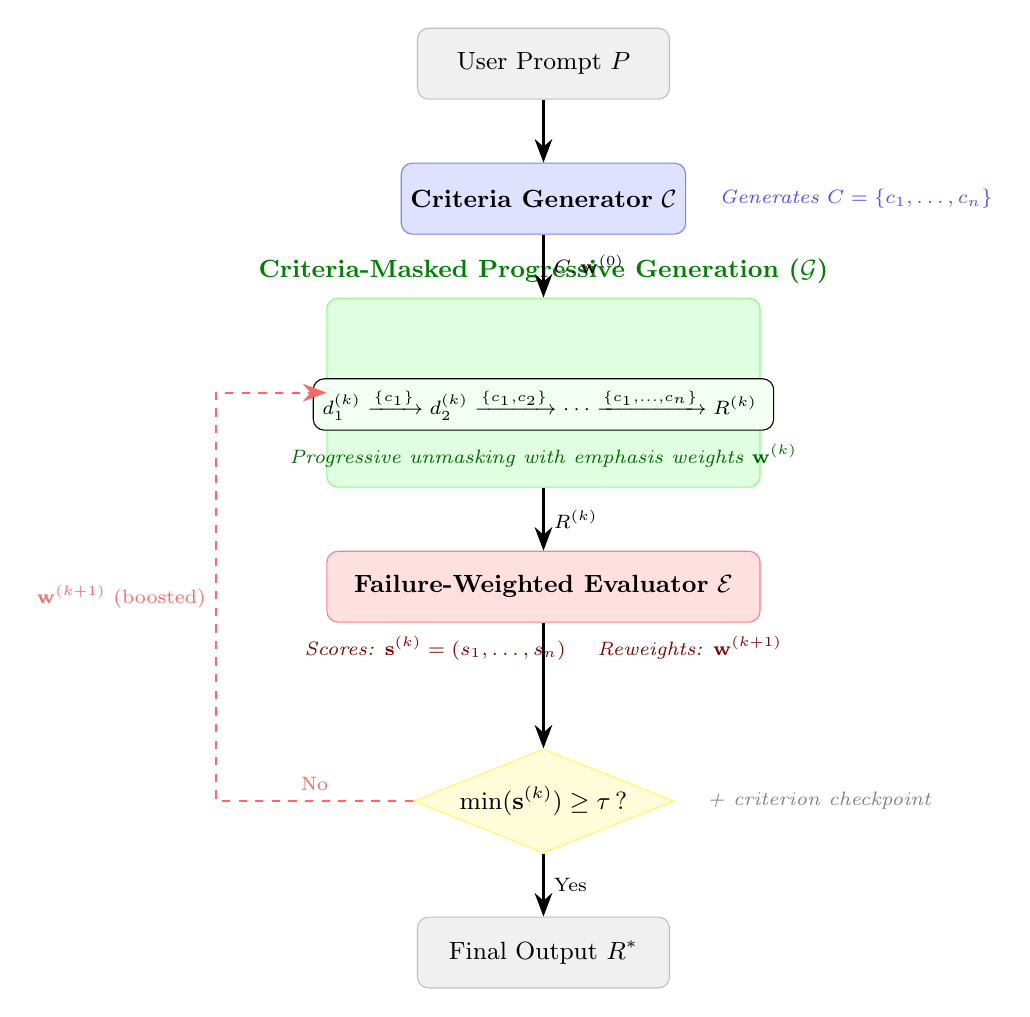
\begin{tikzpicture}[
    node distance=1.0cm and 1.5cm,
    >={Stealth[length=3mm]},
    box/.style={draw, rounded corners, minimum width=3.2cm, minimum height=0.9cm, align=center, font=\small},
    critbox/.style={box, fill=blue!12, draw=blue!50},
    genbox/.style={box, fill=green!12, draw=green!50},
    evalbox/.style={box, fill=red!12, draw=red!50},
    iobox/.style={box, fill=gray!12, draw=gray!50},
    arrow/.style={->, thick},
    dasharrow/.style={->, thick, dashed, red!60},
]

% Input
\node[iobox] (input) {User Prompt $P$};

% Criteria Generator
\node[critbox, below=0.8cm of input] (cg) {\textbf{Criteria Generator} $\calC$};
\node[right=0.3cm of cg, font=\scriptsize\itshape, text=blue!70] (cglabel) {Generates $C = \{c_1, \ldots, c_n\}$};

% CMPG Block
\node[genbox, below=0.8cm of cg, minimum width=5.5cm, minimum height=2.4cm] (cmpgbox) {};
\node[above=0.05cm of cmpgbox.north, font=\small\bfseries, text=green!50!black] {Criteria-Masked Progressive Generation ($\calG$)};

% Sub-steps inside CMPG
\node[draw, rounded corners, fill=green!5, minimum width=4.8cm, minimum height=0.5cm, font=\scriptsize, align=center] at ([yshift=-0.15cm]cmpgbox.center) (sub) {
    $d_1^{(k)} \xrightarrow{\{c_1\}}  d_2^{(k)} \xrightarrow{\{c_1,c_2\}} \cdots \xrightarrow{\{c_1,\ldots,c_n\}} R^{(k)}$
};
\node[below=0.05cm of sub, font=\scriptsize\itshape, text=green!40!black] {Progressive unmasking with emphasis weights $\mathbf{w}^{(k)}$};

% Evaluator
\node[evalbox, below=0.8cm of cmpgbox, minimum width=5.5cm] (eval) {\textbf{Failure-Weighted Evaluator} $\calE$};
\node[below=0.05cm of eval, font=\scriptsize\itshape, text=red!50!black] (evallabel) {Scores: $\mathbf{s}^{(k)} = (s_1, \ldots, s_n)$ \quad Reweights: $\mathbf{w}^{(k+1)}$};

% Decision
\node[draw, diamond, aspect=2.5, below=1.0cm of evallabel, fill=yellow!15, draw=yellow!60, font=\small, align=center, inner sep=1pt] (decide) {$\min(\mathbf{s}^{(k)}) \geq \tau$\,?};

% Output
\node[iobox, below=0.8cm of decide] (output) {Final Output $R^*$};

% Arrows
\draw[arrow] (input) -- (cg);
\draw[arrow] (cg) -- node[right, font=\scriptsize] {$C, \mathbf{w}^{(0)}$} (cmpgbox.north);
\draw[arrow] (cmpgbox.south) -- node[right, font=\scriptsize] {$R^{(k)}$} (eval);
\draw[arrow] (eval) -- (decide);
\draw[arrow] (decide) -- node[right, font=\scriptsize] {Yes} (output);

% Feedback loop
\draw[dasharrow] (decide.west) -- node[above, font=\scriptsize, text=red!60] {No} ++(-2.5,0) |- node[left, font=\scriptsize, text=red!60, near start] {$\mathbf{w}^{(k+1)}$ (boosted)} (cmpgbox.west);

% Checkpoint annotation
\node[right=0.3cm of decide, font=\scriptsize\itshape, text=gray] {+ criterion checkpoint};

\end{tikzpicture}
\caption{\textbf{The Evaluation-First Architecture (\efa{}) pipeline.} A Criteria Generator produces query-specific evaluation criteria before generation begins. The Criteria-Masked Progressive Generator produces a response by incrementally unmasking criteria (analogous to causal token masking but over quality dimensions). The Failure-Weighted Evaluator scores each criterion independently and computes boosted emphasis weights for failing dimensions. The system loops (dashed red arrow) until all criteria pass threshold $\tau$ or maximum iterations are reached. A criterion checkpoint mechanism prevents regression on previously-passing criteria.}
\label{fig:pipeline}
\end{figure}

\subsection{Component 1: Criteria Generator ($\calC$)}

\begin{definition}[Criteria Generator]
Given prompt $P$, the criteria generator $\calC: \mathcal{P} \rightarrow (\calD^n, \R^n)$ produces:
\begin{equation}
    \calC(P) = \left( \{c_1, c_2, \ldots, c_n\}, \; \mathbf{w}^{(0)} \right)
\end{equation}
where each criterion $c_i = (\text{name}_i, \text{definition}_i, \text{rubric}_i)$ consists of a dimension name, a natural language definition, and a scoring rubric mapping scores $\{1, 2, 3, 4, 5\}$ to quality descriptions.
\end{definition}

Criteria are generated dynamically per-query, not from a fixed taxonomy. The generator LLM is prompted to produce non-overlapping, measurable dimensions relevant to the specific prompt. Initial weights are uniform: $w_i^{(0)} = 1/n$ for all $i$.

\textbf{Criteria ordering}: The generator produces criteria in descending order of fundamentality. For example, factual accuracy precedes stylistic polish, as satisfying later criteria is meaningless if fundamental criteria fail. This ordering determines the unmasking sequence in \cmpg{}.

\subsection{Component 2: Criteria-Masked Progressive Generation ($\calG$)}
\label{sec:cmpg}

This is \efa{}'s first novel mechanism. We introduce masking over quality dimensions, analogous to causal masking over token positions in autoregressive transformers.

\begin{definition}[Criteria Mask]
At generation sub-step $j \in \{1, \ldots, n\}$, the criteria mask $M_j \in \{0, 1\}^n$ is defined as:
\begin{equation}
    M_j[i] = \begin{cases} 1 & \text{if } i \leq j \\ 0 & \text{if } i > j \end{cases}
\end{equation}
\end{definition}

\textbf{Progressive generation process}: Rather than presenting all criteria simultaneously, \cmpg{} operates in $n$ sub-steps within each iteration $k$:

\begin{enumerate}[leftmargin=*]
    \item \textbf{Sub-step 1}: Generate draft $d_1^{(k)}$ conditioned on $\{c_1\}$ only (criteria $c_2, \ldots, c_n$ are masked). The generator focuses entirely on the most fundamental quality dimension.
    \item \textbf{Sub-step 2}: Refine $d_1^{(k)}$ into $d_2^{(k)}$ conditioned on $\{c_1, c_2\}$. The generator adjusts the draft to additionally satisfy $c_2$ while maintaining $c_1$.
    \item \textbf{Sub-step $j$}: Refine $d_{j-1}^{(k)}$ into $d_j^{(k)}$ conditioned on $\{c_1, \ldots, c_j\}$ with emphasis weights $\mathbf{w}^{(k)} \odot M_j$.
    \item \textbf{Sub-step $n$}: Final draft $d_n^{(k)} = R^{(k)}$ is conditioned on all criteria.
\end{enumerate}

Formally, at sub-step $j$ of iteration $k$:
\begin{equation}
    d_j^{(k)} = \calG\left(P, \; d_{j-1}^{(k)}, \; \{c_i : M_j[i] = 1\}, \; \mathbf{w}^{(k)} \odot M_j \right)
\end{equation}
where $d_0^{(k)}$ is empty for $k=1$ or the previous iteration's output $R^{(k-1)}$ for $k > 1$.

\textbf{Weight incorporation mechanism}: The emphasis weights $\mathbf{w}^{(k)}$ are incorporated into the generator prompt through \emph{weighted criterion representation}. At each sub-step, the prompt to $\calG$ includes:
\begin{enumerate}[leftmargin=*]
    \item The user prompt $P$.
    \item The current draft $d_{j-1}^{(k)}$ (if available).
    \item Each visible criterion $c_i$ (where $M_j[i] = 1$) annotated with its emphasis level, expressed as a natural language priority directive:
\end{enumerate}

\begin{equation}
    \text{prompt}_j^{(k)} = P \;\|\; d_{j-1}^{(k)} \;\|\; \bigoplus_{i : M_j[i]=1} \left[ \text{priority}(\hat{w}_i^{(k)}) \;\|\; c_i \right]
\label{eq:prompt_construction}
\end{equation}

where $\|$ denotes prompt concatenation, $\oplus$ denotes ordered assembly of criterion blocks, and $\text{priority}(\hat{w}_i^{(k)})$ maps the normalized weight to a natural language emphasis directive:

\begin{equation}
    \text{priority}(w) = \begin{cases}
    \texttt{[CRITICAL---highest priority]} & \text{if } w > 2/n \\
    \texttt{[HIGH---elevated priority]} & \text{if } w > 1.5/n \\
    \texttt{[STANDARD---normal priority]} & \text{if } w \geq 0.5/n \\
    \texttt{[SECONDARY---lower priority]} & \text{if } w < 0.5/n
    \end{cases}
\label{eq:priority}
\end{equation}

Note that all thresholds are defined relative to the uniform weight $1/n$, ensuring consistent behavior regardless of the number of criteria. A criterion receives \texttt{CRITICAL} priority only when its weight exceeds twice the uniform baseline, which occurs after substantial failure-weighted boosting.

This design choice avoids modifying model internals (attention heads, hidden states) and instead operates entirely through prompt engineering, making \efa{} applicable to any LLM accessible via API. Prior work on instruction following \citep{wei2022finetuned} has demonstrated that LLMs are sensitive to emphasis cues and priority ordering within prompts, supporting the effectiveness of structured priority directives for steering generation behavior.

\textbf{Intuition}: This progressive unmasking ensures foundational quality dimensions are satisfied before the generator attempts to optimize for secondary dimensions. It prevents the common failure mode where models optimize for surface-level quality (fluency, style) at the expense of fundamental correctness.

\subsection{Component 3: Failure-Weighted Reattention Loop ($\calE$)}
\label{sec:fwrl}

This is \efa{}'s second novel mechanism. After generating $R^{(k)}$, the evaluator scores it per-criterion and computes reattention weights.

\begin{definition}[Per-Criterion Evaluation]
The evaluator $\calE$ scores the response against each criterion independently:
\begin{equation}
    \mathbf{s}^{(k)} = \calE(R^{(k)}, C) = \left( s_1^{(k)}, s_2^{(k)}, \ldots, s_n^{(k)} \right) \in [0, 1]^n
\end{equation}
where $s_i^{(k)} = \text{score}(R^{(k)}, c_i) / 5$ is the normalized rubric score for criterion $c_i$, obtained by prompting the LLM with the response $R^{(k)}$, criterion $c_i$, and its associated rubric.
\end{definition}

\begin{definition}[Failure-Weighted Reattention]
The emphasis weight for criterion $c_i$ at iteration $k+1$ is updated as:
\begin{equation}
    w_i^{(k+1)} = w_i^{(k)} \cdot \left(1 + \alpha \cdot \max\left(0, \; \tau - s_i^{(k)}\right)\right)
\label{eq:reattention}
\end{equation}
where $\tau \in (0, 1]$ is the passing threshold and $\alpha > 0$ is the reattention strength hyperparameter. Weights are then renormalized: $\hat{w}_i^{(k+1)} = w_i^{(k+1)} / \sum_j w_j^{(k+1)}$.
\end{definition}

\textbf{Properties of Equation~\ref{eq:reattention}}:
\begin{itemize}[leftmargin=*]
    \item \textbf{Passed criteria}: If $s_i^{(k)} \geq \tau$, then $\max(0, \tau - s_i^{(k)}) = 0$ and $w_i^{(k+1)} = w_i^{(k)}$. Weights remain unchanged for satisfied dimensions.
    \item \textbf{Failed criteria}: If $s_i^{(k)} < \tau$, the weight increases proportionally to the severity of failure. A score of $0.2$ with $\tau = 0.6$ produces a larger boost ($\alpha \cdot 0.4$) than a score of $0.5$ ($\alpha \cdot 0.1$).
    \item \textbf{Focal property}: This is analogous to focal loss \citep{lin2017focal}, which down-weights well-classified examples and focuses training on hard negatives. \fwrl{} applies this principle to quality dimensions at inference time rather than training time.
    \item \textbf{Renormalization}: Normalizing to $\sum_i \hat{w}_i = 1$ ensures that boosting failing criteria \emph{relatively} de-emphasizes passing ones, creating a zero-sum reallocation of generation emphasis.
\end{itemize}

\textbf{Criterion checkpoint mechanism}: To prevent regression on previously-passing criteria, we implement a safeguard: if $s_i^{(k+1)} < s_i^{(k)} - \epsilon$ for a criterion that satisfied $s_i^{(k)} \geq \tau$, the system retains the best-observed score for that criterion and marks it as ``locked.'' Locked criteria retain their peak score for convergence tracking and are excluded from further reweighting, ensuring that the reattention mechanism does not destabilize already-satisfactory dimensions. Note that the full response text is not decomposed per-criterion; rather, the locking mechanism prevents the reweighting loop from over-correcting at the expense of previously-passing dimensions. This mechanism is formally integrated into Algorithm~\ref{alg:efa}.

\subsection{Convergence Analysis}
\label{sec:convergence}

We analyze the convergence properties of \efa{} under stated assumptions. We present this as a proposition rather than a theorem, as the key assumption---that LLMs improve on focused criteria---is empirical rather than provable.

\begin{proposition}[Convergence under Focused Improvement]
\label{prop:convergence}
Assume the following two properties hold:
\begin{enumerate}
    \item \textbf{Focused Improvement}: When criterion $c_i$ receives elevated emphasis weight ($\hat{w}_i > 1/n$), the LLM produces output with $s_i^{(k+1)} \geq s_i^{(k)} + \delta$ for some minimum improvement $\delta > 0$.
    \item \textbf{Bounded Regression}: For any criterion $c_i$ with $s_i^{(k)} \geq \tau$, re-generation satisfies $s_i^{(k+1)} \geq \tau - \epsilon$ for regression tolerance $\epsilon < \delta$.
\end{enumerate}
Then the number of failing criteria $|\{i : s_i^{(k)} < \tau\}|$ is non-increasing across iterations, and the system converges (all criteria passing or locked) in at most $K \leq n \cdot \lceil \tau / \delta \rceil$ iterations.
\end{proposition}

\begin{proof}[Proof sketch]
By Bounded Regression, once a criterion passes threshold $\tau$, it either remains above $\tau - \epsilon$ or is locked by the checkpoint mechanism at its passing score. By Focused Improvement, each failing criterion's score increases by at least $\delta$ per iteration. Since scores are bounded in $[0, 1]$ and the maximum distance to threshold is $\tau$, each criterion requires at most $\lceil \tau / \delta \rceil$ iterations to reach $\tau$. With $n$ criteria, the worst case (sequential, non-overlapping improvement) yields $n \cdot \lceil \tau / \delta \rceil$ iterations. In practice, multiple criteria improve simultaneously, yielding substantially faster convergence.
\end{proof}

\textbf{Empirical validation}: The Focused Improvement assumption is supported by the self-refinement literature: \citet{lee2025refinebench} demonstrate that LLMs achieve near-perfect refinement when given targeted, structured feedback about specific quality dimensions. \efa{}'s per-criterion evaluation and emphasis weighting directly provide such structured feedback.

\subsection{Computational Complexity}
\label{sec:complexity}

Let $T$ denote the token cost of a single standard LLM generation call for prompt $P$.

\begin{itemize}[leftmargin=*]
    \item \textbf{Criteria generation}: 1 LLM call $\approx T_C$ tokens (typically $T_C \approx 0.5T$, as criteria are shorter than full responses).
    \item \textbf{Per iteration}: $n$ sub-steps of progressive generation ($n \cdot T$ tokens) + $n$ evaluation calls ($n \cdot T_E$ tokens, where $T_E \approx 0.3T$ per criterion).
    \item \textbf{Total over $K$ iterations}: $T_C + K \cdot n \cdot (T + T_E)$.
\end{itemize}

\textbf{Worst-case cost}: With $n = 5$ criteria, $K_{\max} = 3$ iterations, and $T_E = 0.3T$:
\begin{equation}
    T_{\text{EFA}} \approx 0.5T + 3 \cdot 5 \cdot (T + 0.3T) = 0.5T + 19.5T = 20T
\end{equation}

This represents a $20\times$ cost increase over single-pass generation. This is comparable to Best-of-20 sampling and lower than full multi-agent debate pipelines (which typically require $30{-}50T$). The cost is justified when output quality and reliability are prioritized over latency---common in enterprise, medical, legal, and high-stakes generation settings.

\textbf{Cost reduction strategies}: (a) \emph{Adaptive sub-stepping}: Skip sub-steps for criteria with high initial scores. (b) \emph{Early termination}: Exit the loop when all criteria pass after any sub-step, not only after the full iteration. (c) \emph{Batched evaluation}: Score all criteria in a single LLM call with multi-dimensional rubric prompting, reducing the $n \cdot T_E$ term to $\approx 1.5 T_E$.

\subsection{Complete Algorithm}

\begin{algorithm}[H]
\caption{Evaluation-First Architecture (\efa{})}
\label{alg:efa}
\begin{algorithmic}[1]
\REQUIRE User prompt $P$, threshold $\tau$, max iterations $K_{\max}$, reattention strength $\alpha$, regression tolerance $\epsilon$
\ENSURE Response $R^*$
\STATE $C, \mathbf{w}^{(0)} \leftarrow \calC(P)$ \COMMENT{Generate criteria}
\STATE $R^{(0)} \leftarrow \emptyset$; \; $\text{locked} \leftarrow \emptyset$; \; $\mathbf{s}_{\text{best}} \leftarrow \mathbf{0}$
\FOR{$k = 1$ to $K_{\max}$}
    \STATE \COMMENT{\textbf{--- Criteria-Masked Progressive Generation ---}}
    \STATE $d_0^{(k)} \leftarrow R^{(k-1)}$
    \FOR{$j = 1$ to $|C|$}
        \STATE $M_j \leftarrow \text{CausalCriteriaMask}(j, |C|)$
        \STATE Construct prompt per Eq.~\ref{eq:prompt_construction} with priorities per Eq.~\ref{eq:priority}
        \STATE $d_j^{(k)} \leftarrow \calG(P, \; d_{j-1}^{(k)}, \; C \odot M_j, \; \hat{\mathbf{w}}^{(k-1)} \odot M_j)$
    \ENDFOR
    \STATE $R^{(k)} \leftarrow d_{|C|}^{(k)}$
    \STATE
    \STATE \COMMENT{\textbf{--- Per-Criterion Evaluation ---}}
    \STATE $\mathbf{s}^{(k)} \leftarrow \calE(R^{(k)}, C)$
    \STATE
    \STATE \COMMENT{\textbf{--- Criterion Checkpoint ---}}
    \FOR{$i = 1$ to $|C|$}
        \IF{$i \in \text{locked}$}
            \STATE $s_i^{(k)} \leftarrow s_{\text{best},i}$ \COMMENT{Retain locked score}
        \ELSIF{$s_{\text{best},i} \geq \tau$ \AND $s_i^{(k)} < s_{\text{best},i} - \epsilon$}
            \STATE $\text{locked} \leftarrow \text{locked} \cup \{i\}$ \COMMENT{Lock regressed criterion}
            \STATE $s_i^{(k)} \leftarrow s_{\text{best},i}$
        \ELSE
            \STATE $s_{\text{best},i} \leftarrow \max(s_{\text{best},i}, \; s_i^{(k)})$
        \ENDIF
    \ENDFOR
    \STATE
    \IF{$\min(\mathbf{s}^{(k)}) \geq \tau$}
        \RETURN $R^{(k)}$ \COMMENT{All criteria satisfied}
    \ENDIF
    \STATE
    \STATE \COMMENT{\textbf{--- Failure-Weighted Reattention ---}}
    \FOR{$i = 1$ to $|C|$}
        \IF{$i \notin \text{locked}$}
            \STATE $w_i^{(k)} \leftarrow w_i^{(k-1)} \cdot (1 + \alpha \cdot \max(0, \; \tau - s_i^{(k)}))$
        \ENDIF
    \ENDFOR
    \STATE $\hat{\mathbf{w}}^{(k)} \leftarrow \text{Normalize}(\mathbf{w}^{(k)})$
\ENDFOR
\RETURN $R^{(K_{\max})}$
\end{algorithmic}
\end{algorithm}

% ============================================================================
% 4. EXPERIMENTAL SETUP
% ============================================================================
\section{Experimental Design}
\label{sec:experiments}

\subsection{Baselines}

We compare \efa{} against the following seven baselines, designed to isolate the contribution of each architectural component:

\begin{enumerate}[leftmargin=*]
    \item \textbf{Single-pass}: Standard LLM generation without criteria or refinement. Measures the baseline quality achievable without any architectural intervention.
    \item \textbf{Self-Refine} \citep{madaan2023selfrefine}: Iterative holistic self-feedback and refinement. The primary comparison for iterative improvement without criteria structure.
    \item \textbf{Rubric-then-Score}: Generate criteria (same as \efa{} Step 1), generate response without criteria conditioning, then score with the rubric. Tests whether criteria-aware generation outperforms criteria-unaware generation followed by the same evaluation.
    \item \textbf{All-Criteria-at-Once}: Provide all criteria simultaneously to the generator in a single pass (no progressive masking, no iteration). Tests whether \cmpg{}'s progressive unmasking adds value over naive full-criteria prompting.
    \item \textbf{Uniform Reattention}: Generate with criteria, evaluate per-criterion, but re-generate with uniform weights on failure (no failure weighting). Tests whether \fwrl{}'s targeted reweighting outperforms uniform retry.
    \item \textbf{Best-of-$N$}: Generate $N$ independent responses (each with full criteria conditioning), evaluate all, return the highest-scoring candidate. Tests whether \efa{}'s iterative refinement outperforms brute-force sampling at comparable or lower token cost.
    \item \textbf{FusioN} \citep{agarwal2025fusion}: Multi-candidate synthesis without criteria guidance. Represents the state-of-the-art in inference-time quality scaling.
\end{enumerate}

\subsection{Ablation Studies}

To validate each component's individual contribution, we conduct four ablation conditions:
\begin{enumerate}[leftmargin=*]
    \item \textbf{$-$DynCriteria}: Replace dynamic per-query criteria with a fixed universal set of five criteria (relevance, accuracy, completeness, clarity, conciseness). Tests the value of dynamic criteria generation.
    \item \textbf{$-$\cmpg{}}: Remove progressive masking; present all criteria at once in every sub-step. Tests whether progressive unmasking improves over simultaneous conditioning.
    \item \textbf{$-$\fwrl{}}: Remove failure weighting; use uniform weights across all iterations. Tests whether targeted reweighting outperforms uniform iteration.
    \item \textbf{$-$Iteration}: Single generation pass with all criteria (no refinement loop). Tests whether iteration adds value beyond single-pass criteria-conditioned generation.
\end{enumerate}

\subsection{Evaluation Metrics}

\begin{itemize}[leftmargin=*]
    \item \textbf{Rubric Adherence Score (RAS)}: Mean per-criterion score across all criteria, averaged over test prompts. Range: $[0, 1]$.
    \item \textbf{All-Pass Rate (APR)}: Percentage of test prompts where all criteria meet threshold $\tau$. Measures reliability.
    \item \textbf{Iterations to Convergence (ITC)}: Mean number of iterations before all criteria pass or maximum reached. Measures efficiency.
    \item \textbf{Total Token Cost (TTC)}: Total tokens consumed across the full pipeline. Measures computational efficiency.
\end{itemize}

\subsection{Hyperparameter Settings}

Based on preliminary analysis, we use the following default configuration: $n = 5$ criteria per query, threshold $\tau = 0.6$ (corresponding to rubric score $\geq 3/5$), maximum iterations $K_{\max} = 3$, reattention strength $\alpha = 2.0$, and regression tolerance $\epsilon = 0.1$. For Best-of-$N$, we use $N = 5$.

\subsection{Experimental Setup}

\textbf{Benchmark.} We use MT-Bench \citep{zheng2023judging}, a curated set of 80 multi-turn prompts spanning 8 categories: writing, roleplay, extraction, reasoning, math, coding, knowledge (STEM), and knowledge (humanities/social science). MT-Bench is widely adopted for evaluating LLM quality and provides diverse task types that stress-test \efa{}'s generality.

\textbf{Cross-model evaluation.} To eliminate self-preference bias---a known confound in LLM-as-Judge evaluation \citep{zheng2023judging}---we use separate models for generation and evaluation from different model families:
\begin{itemize}[leftmargin=*]
    \item \textbf{Generator}: MiniMax-M2.5 (commercial cloud API via OpenAI-compatible endpoint)
    \item \textbf{Evaluator}: Qwen-3.5-9B running locally via Ollama (open-source, different architecture)
\end{itemize}

This cross-family design ensures that the evaluator has no systematic preference for the generator's outputs, strengthening the validity of per-criterion scores. The same generator--evaluator pair is used across all methods for fair comparison.

\textbf{Scale.} Each of the 12 methods (7 baselines + 4 ablations + full \efa{}) is evaluated on all 80 prompts, yielding 960 total experimental runs with over 1.3 million tokens consumed.

% ============================================================================
% 5. EXPERIMENTAL RESULTS
% ============================================================================
\section{Experimental Results}
\label{sec:results}

\subsection{Main Results}

Table~\ref{tab:main_results} presents the full results across all 12 methods on 80 MT-Bench prompts. \efa{} achieves the highest All-Pass Rate (96.2\%) among all methods, outperforming every baseline.

\begin{table}[t]
\centering
\caption{\textbf{Main results on MT-Bench (80 prompts).} Generator: MiniMax-M2.5; Evaluator: Qwen-3.5-9B (Ollama). RAS = Rubric Adherence Score (mean), APR = All-Pass Rate (\%), ITC = Iterations to Convergence (mean), TTC = Total Token Cost (mean). Best result per metric in \textbf{bold}. $\dagger$ denotes ablation variants.}
\label{tab:main_results}
\small
\begin{tabular}{@{}lcccc@{}}
\toprule
\textbf{Method} & \textbf{RAS} $\uparrow$ & \textbf{APR (\%)} $\uparrow$ & \textbf{ITC} $\downarrow$ & \textbf{TTC} $\downarrow$ \\
\midrule
\multicolumn{5}{l}{\textit{Baselines}} \\
\quad Single-pass           & 0.881 & 71.2 & \textbf{1.0} & \textbf{9,210} \\
\quad Rubric-then-Score     & 0.863 & 72.5 & 1.0 & 9,469 \\
\quad All-Criteria-at-Once  & 0.925 & 90.0 & 1.3 & 13,408 \\
\quad Uniform Reattention   & 0.935 & 90.0 & 1.3 & 17,814 \\
\quad Best-of-5             & 0.957 & 91.2 & 1.0 & 21,999 \\
\quad Self-Refine           & 0.953 & 92.5 & 1.4 & 13,652 \\
\quad FusioN                & 0.956 & 92.5 & 1.0 & 15,449 \\
\midrule
\multicolumn{5}{l}{\textit{Ablations}$^\dagger$} \\
\quad EFA $-$Iteration      & 0.943 & 83.8 & 1.0 & 15,652 \\
\quad EFA $-$DynCriteria    & 0.943 & 88.8 & 1.4 & 18,378 \\
\quad EFA $-$\cmpg{}        & 0.950 & 92.5 & 1.3 & 14,579 \\
\quad EFA $-$\fwrl{}        & \textbf{0.967} & \textbf{96.2} & 1.1 & 17,524 \\
\midrule
\textbf{\efa{} (Full)}      & 0.962 & \textbf{96.2} & 1.2 & 16,449 \\
\bottomrule
\end{tabular}
\end{table}

\begin{figure}[t]
\centering
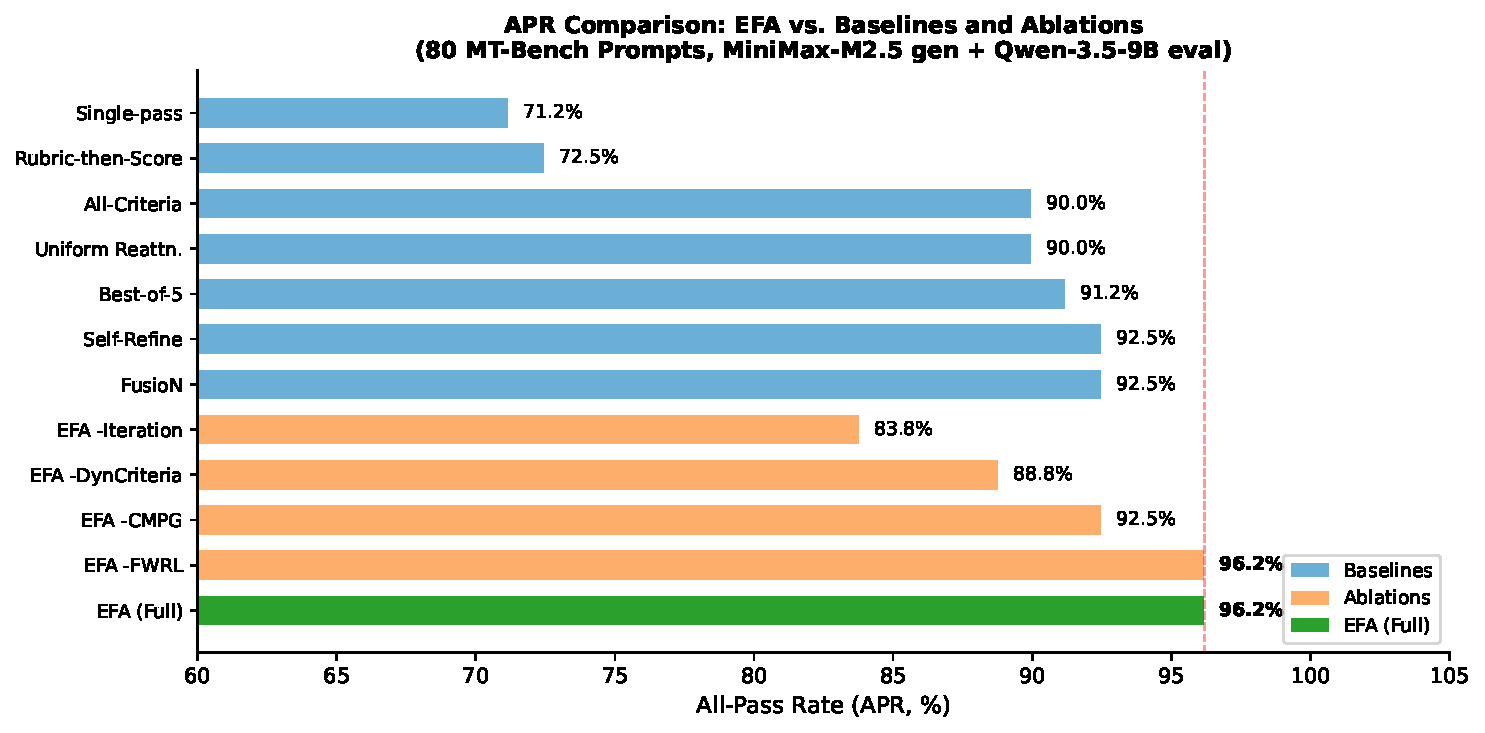
\includegraphics[width=\textwidth]{figures/apr_comparison.pdf}
\caption{\textbf{APR comparison across all 12 methods} on 80 MT-Bench prompts with cross-model evaluation (MiniMax-M2.5 generator, Qwen-3.5-9B evaluator). \efa{} and \efa{} $-$\fwrl{} both achieve 96.2\% APR, outperforming all seven baselines. The dashed red line marks the \efa{} APR.}
\label{fig:apr_comparison}
\end{figure}

\textbf{Key findings.}\footnote{APR percentages are rounded to one decimal place; percentage-point deltas are computed from the displayed values.} (1)~\efa{} achieves 96.2\% APR, a +25.0 percentage point (pp) improvement over single-pass and +3.7pp over the strongest baselines (Self-Refine and FusioN at 92.5\%). Notably, the \efa{} $-$\fwrl{} ablation matches this 96.2\% APR with slightly higher RAS (0.967 vs.\ 0.962), indicating that failure-weighted reattention does not contribute measurably on this benchmark (see Section~\ref{sec:fwrl_analysis}). (2)~\efa{} outperforms Best-of-5 by +5.0pp APR while using approximately 75\% of its token budget, demonstrating that targeted iterative refinement is more token-efficient than brute-force sampling. (3)~Even criteria-aware baselines that do not iterate (All-Criteria-at-Once, 90.0\%) substantially underperform \efa{}, confirming that the iterative refinement loop is essential. (4)~Rubric-then-Score (0.863 RAS) scores lower than single-pass (0.881 RAS) because per-criterion evaluation with specific rubrics is more demanding than holistic scoring---the same response receives lower scores when evaluated against granular quality dimensions.

\subsection{Ablation Analysis}

The ablation study reveals the contribution of each \efa{} component by measuring the APR drop when removing it:

\begin{itemize}[leftmargin=*]
    \item \textbf{Iteration} ($-12.4$pp): The largest contributor. Without iterative refinement, APR drops from 96.2\% to 83.8\%. This confirms that multi-pass generation with criterion-level feedback is essential---a single criteria-conditioned pass is insufficient.
    \item \textbf{Dynamic Criteria} ($-7.4$pp): Replacing per-query criteria with a fixed universal set drops APR from 96.2\% to 88.8\%. Dynamic, query-specific criteria provide meaningfully better guidance than generic dimensions.
    \item \textbf{\cmpg{} (Progressive Masking)} ($-3.7$pp): Removing progressive unmasking drops APR from 96.2\% to 92.5\%. The progressive curriculum over quality dimensions provides a measurable gain over presenting all criteria simultaneously.
    \item \textbf{\fwrl{} (Failure-Weighted Reattention)} ($0.0$pp): Removing failure-proportional reweighting yields identical APR (96.2\%) and slightly \emph{higher} RAS (0.967 vs.\ 0.962). We analyze this finding in detail below.
\end{itemize}

\begin{figure}[t]
\centering
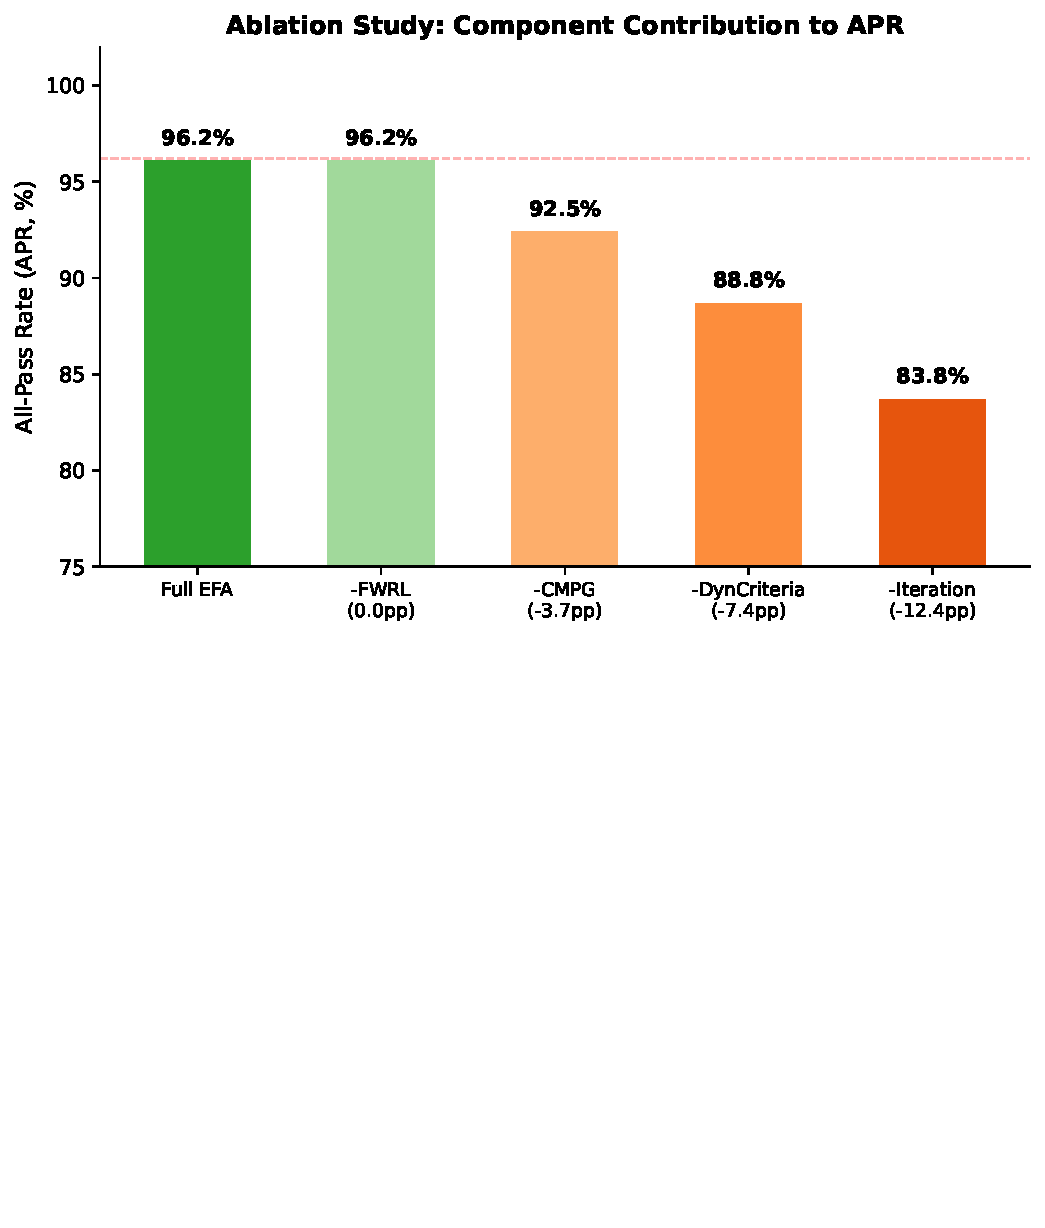
\includegraphics[width=0.85\textwidth]{figures/ablation_waterfall.pdf}
\caption{\textbf{Ablation study: component contribution to APR.} Removing iteration causes the largest drop ($-12.4$pp), followed by dynamic criteria ($-7.4$pp) and \cmpg{} ($-3.7$pp). Removing \fwrl{} yields no measurable change ($0.0$pp).}
\label{fig:ablation}
\end{figure}

\subsection{Analysis of \fwrl{}'s Marginal Contribution}
\label{sec:fwrl_analysis}

The absence of measurable \fwrl{} contribution warrants careful discussion, as failure-weighted reattention is a theoretically motivated component of our framework.

\textbf{Ceiling effect hypothesis.} MiniMax-M2.5 is a strong commercial model that, when given explicit criteria and iterative feedback, achieves near-perfect scores on most criteria after the first iteration. With few criteria failing after iteration 1, \fwrl{}'s reweighting mechanism has little signal to amplify. The uniform reattention baseline (90.0\% APR) is substantially lower than full \efa{} (96.2\%), but this gap reflects the absence of dynamic criteria and \cmpg{} in that baseline---not weight distribution. The $-$\fwrl{} ablation (96.2\% APR, identical to full \efa{}) is the direct test of failure weighting's contribution, and it confirms that weight distribution does not matter on this benchmark.

\textbf{When \fwrl{} should matter.} We hypothesize that \fwrl{}'s contribution increases when: (a)~the generator is weaker (producing more per-criterion failures that create meaningful weight differentials), (b)~prompts are harder (requiring more iterations with heterogeneous failure patterns), or (c)~criteria counts are larger (creating more opportunities for dimension-specific bottlenecks). Testing these conditions is an important direction for future work.

\textbf{Theoretical value.} Even when empirically marginal, \fwrl{} provides a principled mechanism for allocating generation emphasis that degrades gracefully: when all criteria pass, weights remain uniform and the mechanism is a no-op. It adds no cost when unnecessary and provides targeted remediation when criterion failures are heterogeneous.

\subsection{Efficiency Analysis}

Table~\ref{tab:main_results} reveals an important cost-quality tradeoff. \efa{} achieves its 96.2\% APR at a mean cost of 16,449 tokens---1.8$\times$ the single-pass cost of 9,210 tokens but only 0.75$\times$ the Best-of-5 cost of 21,999 tokens. The \efa{} pipeline's iterative architecture is more token-efficient than brute-force sampling because it \emph{diagnoses and targets} specific failure dimensions rather than regenerating the entire response.

Self-Refine achieves 92.5\% APR at 13,652 tokens (0.83$\times$ \efa{}), offering a reasonable cost-quality tradeoff when the 3.7pp APR gap is acceptable. For applications demanding the highest reliability, \efa{}'s additional investment yields the best observed APR. Figure~\ref{fig:cost_quality} visualizes this tradeoff.

\begin{figure}[t]
\centering
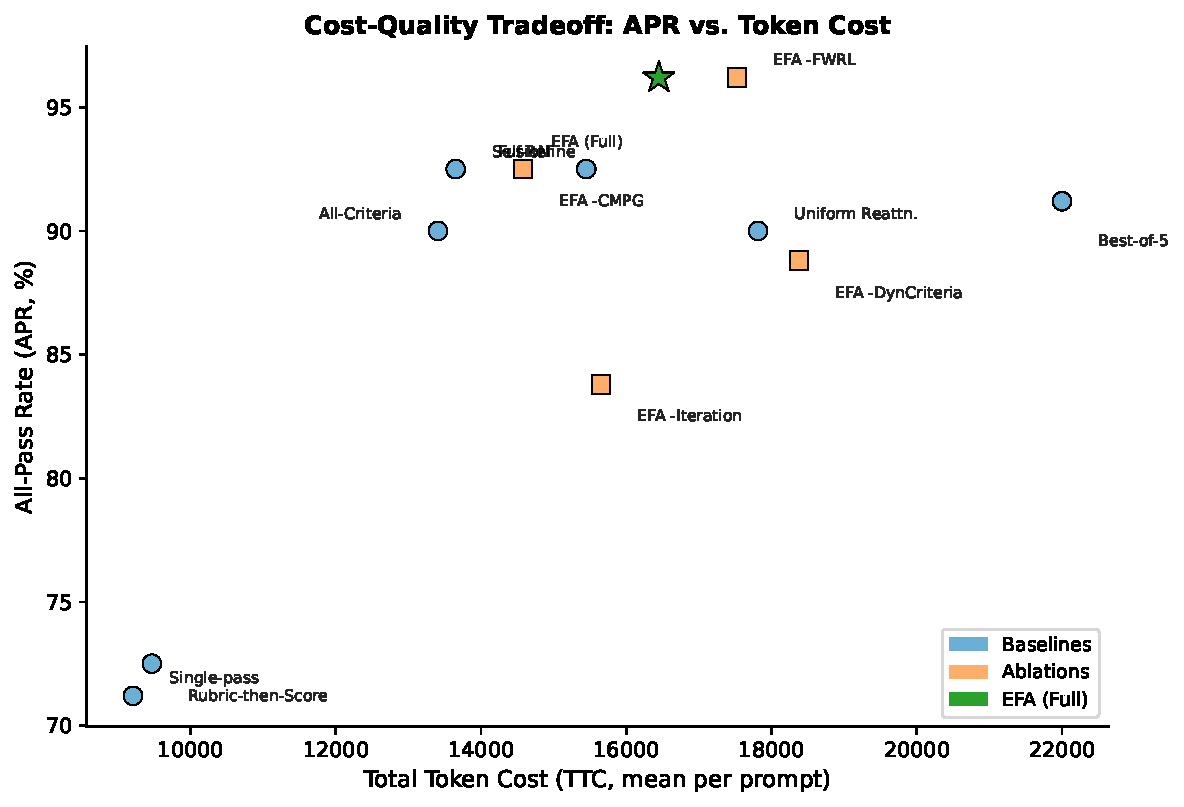
\includegraphics[width=0.85\textwidth]{figures/cost_quality_scatter.pdf}
\caption{\textbf{Cost-quality tradeoff.} Each point represents a method's mean APR vs.\ mean token cost per prompt. \efa{} (green star) achieves the highest APR tier at moderate cost---more efficient than Best-of-5 and comparable to FusioN/Self-Refine in cost while delivering higher reliability.}
\label{fig:cost_quality}
\end{figure}

% ============================================================================
% 6. ANALYSIS AND DISCUSSION
% ============================================================================
\section{Analysis and Discussion}

\subsection{Why Evaluation-First Outperforms Evaluate-After}

The core insight supporting \efa{} comes from the self-refinement literature: structured, targeted feedback enables near-perfect refinement, while self-diagnosis is the bottleneck \citep{lee2025refinebench}. \efa{} eliminates the self-diagnosis problem entirely by pre-specifying what success looks like before generation begins. The model never needs to ``figure out what went wrong''---the per-criterion evaluation tells it exactly which dimensions failed and by how much.

Our experimental results directly validate this insight: the +25.0pp APR improvement over single-pass (71.2\% $\rightarrow$ 96.2\%) demonstrates that criteria awareness dramatically improves output quality. The +3.7pp gain over Self-Refine (92.5\% $\rightarrow$ 96.2\%) further confirms that structured per-criterion feedback outperforms holistic textual feedback.

\subsection{The Focal Property of Failure-Weighted Reattention}

\fwrl{} implements an inference-time analog of focal loss \citep{lin2017focal}. In object detection, focal loss down-weights well-classified examples to focus training on hard negatives. \fwrl{} analogously de-emphasizes (relatively) well-satisfied criteria to focus generation compute on failing dimensions.

Our MT-Bench experiments show that \fwrl{}'s contribution is empirically marginal when paired with a strong generator (Section~\ref{sec:fwrl_analysis}). We attribute this to a ceiling effect: MiniMax-M2.5 rarely produces heterogeneous per-criterion failures that would create meaningful weight differentials. This does not invalidate the mechanism---it indicates that the current benchmark does not sufficiently stress-test it. The theoretical efficiency property (allocating more generation budget to failing dimensions) remains sound and is expected to manifest with weaker generators or harder tasks where per-criterion failure rates vary more widely.

\subsection{Criteria Masking as Quality Curriculum}

\cmpg{}'s progressive unmasking implements a form of curriculum learning \citep{bengio2009curriculum} at inference time. By satisfying fundamental criteria before introducing secondary ones, the generator builds a solid foundation that subsequent refinements can improve without undermining. This prevents the common failure mode of surface-level optimization at the expense of deep quality---analogous to how curriculum learning in training prevents models from memorizing surface patterns before learning fundamental structure.

\subsection{Limitations}

\begin{itemize}[leftmargin=*]
    \item \textbf{Criteria quality dependence}: \efa{}'s effectiveness is bounded by the quality of generated criteria. Poor, overlapping, or irrelevant criteria degrade the entire pipeline. Criteria quality could be improved through the rubric refinement techniques of \citet{wang2026rrd}.
    \item \textbf{Compute cost}: With worst-case $20T$ token cost for $n=5$, $K=3$, \efa{} is not suitable for latency-sensitive applications. The cost reduction strategies in \S\ref{sec:complexity} partially address this, but a fundamental tradeoff between quality and cost remains.
    \item \textbf{Conflicting criteria}: When criteria inherently conflict (e.g., conciseness vs.\ completeness), failure-weighted reattention may oscillate between dimensions. The criterion checkpoint mechanism mitigates oscillation but may converge to a Pareto-suboptimal solution that satisfies each dimension at only the threshold level.
    \item \textbf{Evaluator reliability}: Per-criterion scoring is performed by an LLM judge, inheriting known biases of LLM-as-a-Judge approaches (position bias, verbosity bias, self-preference bias). Our cross-model design (MiniMax generator, Qwen evaluator) mitigates self-preference bias but does not eliminate all evaluator limitations.
    \item \textbf{\fwrl{} ceiling effect}: Our experiments show that failure-weighted reattention provides no measurable improvement over uniform reweighting on MT-Bench with a strong generator. The mechanism's contribution is expected to increase with weaker generators, harder benchmarks, or larger criteria counts---conditions that produce more heterogeneous per-criterion failure patterns. Validating this hypothesis across generator capabilities and task difficulties is important future work.
    \item \textbf{Prompt sensitivity}: Our results are based on a single set of prompt templates (Appendix~\ref{app:prompts}); sensitivity to prompt wording has not been evaluated. LLM performance is known to vary with prompt formulation, and the effectiveness of priority directives (Eq.~\ref{eq:priority}) may depend on specific phrasing choices.
    \item \textbf{Statistical significance}: With 80 prompts, the top-3 gap (EFA at 96.2\% vs.\ Self-Refine/FusioN at 92.5\%) corresponds to a difference of 3 prompts. Future work should report bootstrap confidence intervals or McNemar tests to quantify significance.
    \item \textbf{Prompt-level conditioning}: The current design operates through prompt engineering (Eq.~\ref{eq:prompt_construction}) rather than modifying model internals. While this maximizes applicability across API-accessible models, a deeper integration at the embedding or attention level could yield stronger conditioning effects. This is an intentional design tradeoff: the framework's value is demonstrable without any model-weight access.
\end{itemize}

% ============================================================================
% 7. CONCLUSION
% ============================================================================
\section{Conclusion}

We presented \textbf{Evaluation-First Architecture} (\efa{}), a prompt-level generation framework that inverts the traditional generate-then-evaluate paradigm by generating evaluation criteria before generation and using them as structured conditioning targets. Evaluated on 80 MT-Bench prompts with cross-model evaluation (MiniMax-M2.5 generator, Qwen-3.5-9B evaluator), \efa{} achieves 96.2\% All-Pass Rate---a +25.0pp improvement over single-pass generation and +3.7pp over the strongest baselines (Self-Refine and FusioN).

Our ablation study identifies \textbf{iteration} ($-12.4$pp) and \textbf{dynamic criteria generation} ($-7.4$pp) as the primary drivers of \efa{}'s effectiveness, with \textbf{\cmpg{}} contributing a meaningful $+3.7$pp gain. We transparently report that \textbf{\fwrl{}'s failure-proportional reweighting} shows no measurable improvement over uniform reweighting on this benchmark---an ablation without \fwrl{} achieves identical APR (96.2\%) and slightly higher RAS (0.967 vs.\ 0.962)---which we attribute to a ceiling effect with a strong generator.

The core insight is validated: \emph{LLMs produce substantially better output when they know what ``good'' looks like before they start writing.} \efa{} transforms evaluation from a passive post-hoc measurement into an active generation specification, drawing a direct analogy to test-driven development in software engineering.

\textbf{Reproducibility.} Code, experiment configurations, prompt templates, and all 960 result JSONs are available at \url{https://github.com/karthyick/evaluation-first-attention}.

Future work includes: (a)~validating \fwrl{}'s contribution with weaker generators and harder benchmarks where per-criterion failure heterogeneity is greater, (b)~deeper model integration via criteria embeddings in the attention mechanism, (c)~adaptive criteria count selection based on prompt complexity, and (d)~domain-specific evaluation in code generation, medical question answering, and enterprise document synthesis.

% ============================================================================
% REFERENCES
% ============================================================================
\bibliographystyle{plainnat}

\begin{thebibliography}{99}

\bibitem[Madaan et al.(2023)]{madaan2023selfrefine}
Aman Madaan, Niket Tandon, Prakhar Gupta, Skyler Hallinan, Luyu Gao, Sarah Wiegreffe, Uri Alon, Nouha Dziri, Shrimai Prabhumoye, Yiming Yang, Shashank Gupta, Bodhisattwa Prasad Majumder, Katherine Hermann, Sean Welleck, Amir Yazdanbakhsh, and Peter Clark.
\newblock Self-Refine: Iterative Refinement with Self-Feedback.
\newblock In \emph{Advances in Neural Information Processing Systems (NeurIPS)}, 2023.

\bibitem[Shinn et al.(2023)]{shinn2023reflexion}
Noah Shinn, Federico Cassano, Ashwin Gopinath, Karthik Narasimhan, and Shunyu Yao.
\newblock Reflexion: Language Agents with Verbal Reinforcement Learning.
\newblock In \emph{Advances in Neural Information Processing Systems (NeurIPS)}, 2023.

\bibitem[Gou et al.(2024)]{gou2024critic}
Zhibin Gou, Zhihong Shao, Yeyun Gong, Yelong Shen, Yujiu Yang, Nan Duan, and Weizhu Chen.
\newblock CRITIC: Large Language Models Can Self-Correct with Tool-Interactive Critiquing.
\newblock In \emph{International Conference on Learning Representations (ICLR)}, 2024.

\bibitem[Liu et al.(2023)]{liu2023geval}
Yang Liu, Dan Iter, Yichong Xu, Shuohang Wang, Ruochen Xu, and Chenguang Zhu.
\newblock G-Eval: NLG Evaluation using GPT-4 with Better Human Alignment.
\newblock In \emph{Proceedings of the 2023 Conference on Empirical Methods in Natural Language Processing (EMNLP)}, 2023.

\bibitem[Jiang et al.(2023)]{jiang2023llmblender}
Dongfu Jiang, Xiang Ren, and Bill Yuchen Lin.
\newblock LLM-Blender: Ensembling Large Language Models with Pairwise Ranking and Generative Fusion.
\newblock In \emph{Proceedings of the 61st Annual Meeting of the Association for Computational Linguistics (ACL)}, 2023.

\bibitem[Lin et al.(2017)]{lin2017focal}
Tsung-Yi Lin, Priya Goyal, Ross Girshick, Kaiming He, and Piotr Doll\'{a}r.
\newblock Focal Loss for Dense Object Detection.
\newblock In \emph{IEEE International Conference on Computer Vision (ICCV)}, 2017.

\bibitem[Bengio et al.(2009)]{bengio2009curriculum}
Yoshua Bengio, J\'{e}r\^{o}me Louradour, Ronan Collobert, and Jason Weston.
\newblock Curriculum Learning.
\newblock In \emph{International Conference on Machine Learning (ICML)}, 2009.

\bibitem[Bai et al.(2022)]{bai2022constitutional}
Yuntao Bai, Saurav Kadavath, Sandipan Kundu, Amanda Askell, Jackson Kernion, Andy Jones, Anna Chen, Anna Goldie, Azalia Mirhoseini, Cameron McKinnon, et al.
\newblock Constitutional AI: Harmlessness from AI Feedback.
\newblock \emph{arXiv preprint arXiv:2212.08073}, 2022.

\bibitem[Yang and Klein(2021)]{yang2021fudge}
Kevin Yang and Dan Klein.
\newblock FUDGE: Controlled Text Generation With Future Discriminators.
\newblock In \emph{Proceedings of the 2021 Conference of the North American Chapter of the Association for Computational Linguistics (NAACL)}, 2021.

\bibitem[Dathathri et al.(2020)]{dathathri2020plug}
Sumanth Dathathri, Andrea Madotto, Janice Lan, Jane Hung, Eric Frank, Piero Molino, Jason Yosinski, and Rosanne Liu.
\newblock Plug and Play Language Models: A Simple Approach to Controlled Text Generation.
\newblock In \emph{International Conference on Learning Representations (ICLR)}, 2020.

\bibitem[Ho and Salimans(2022)]{ho2022classifier}
Jonathan Ho and Tim Salimans.
\newblock Classifier-Free Diffusion Guidance.
\newblock In \emph{NeurIPS 2021 Workshop on Deep Generative Models and Downstream Applications}, 2022.

\bibitem[Chen et al.(2025)]{chen2025magicore}
Justin Chih-Yao Chen, Archiki Prasad, Swarnadeep Saha, and Mohit Bansal.
\newblock MAgICoRe: Multi-Agent, Iterative, Coarse-to-Fine Refinement for Reasoning.
\newblock In \emph{Proceedings of the 2025 Conference on Empirical Methods in Natural Language Processing (EMNLP)}, 2025.

\bibitem[Lee et al.(2025)]{lee2025refinebench}
Hyunseok Lee, Seunghyuk Oh, Jaehyung Kim, Jinwoo Shin, and Jihoon Tack.
\newblock RefineBench: Evaluating Self-Refinement Capabilities of Large Language Models.
\newblock \emph{arXiv preprint arXiv:2411.00548}, 2025.

\bibitem[Agarwal et al.(2025)]{agarwal2025fusion}
Rishabh Agarwal, Nino Vieillard, Yongchao Zhou, Avi Singh, and Olivier Bachem.
\newblock Making, not Taking, the Best of N.
\newblock \emph{arXiv preprint arXiv:2510.00931}, 2025.

\bibitem[Li et al.(2025)]{li2025openrubrics}
Tianyi Li, Tong Xiao, Zhixian Zhang, et al.
\newblock OpenRubrics: Towards Scalable Synthetic Rubric Generation for Reward Modeling and LLM Alignment.
\newblock \emph{arXiv preprint arXiv:2510.07743}, 2025.

\bibitem[Zhang et al.(2025)]{zhang2025carmo}
Zhiyu Zhang, Shujian Huang, Xue Han, and Jiajun Chen.
\newblock CARMO: Dynamic Criteria Generation for Context-Aware Reward Modelling.
\newblock In \emph{Findings of the Association for Computational Linguistics: ACL 2025}, 2025.

\bibitem[Wang et al.(2026)]{wang2026rrd}
Yufei Wang, Jiayi Pan, Yaswanth Narsupalli, Tong Zhang, and Yulia Tsvetkov.
\newblock Rethinking Rubric Generation for Improving LLM Judge and Reward Modeling for Open-ended Tasks.
\newblock \emph{arXiv preprint arXiv:2602.05125}, 2026.

\bibitem[Chen et al.(2025b)]{chen2025autoscore}
Mengxiao Chen, Yunfei Wang, Yanqing Wang, et al.
\newblock AutoSCORE: Enhancing Automated Scoring with Multi-Agent Large Language Models via Structured Component Recognition.
\newblock \emph{arXiv preprint arXiv:2509.21910}, 2025.

\bibitem[Ravi et al.(2025)]{ravi2025llmloop}
Karandeep Ravi, Valerio Terragni, and Gunel Jahangirova.
\newblock LLMLOOP: Improving LLM-Generated Code and Tests via Iterative Feedback.
\newblock In \emph{IEEE International Conference on Software Maintenance and Evolution (ICSME)}, 2025.

\bibitem[Khattab et al.(2023)]{khattab2023dspy}
Omar Khattab, Arnav Singhvi, Paridhi Maheshwari, Zhiyuan Zhang, Keshav Santhanam, Sri Vardhamanan, Saiful Haq, Ashutosh Sharma, Thomas T. Joshi, Moez Moez, Hanna Hajishirzi, and Christopher Potts.
\newblock DSPy: Compiling Declarative Language Model Calls into Self-Improving Pipelines.
\newblock In \emph{International Conference on Learning Representations (ICLR)}, 2024.

\bibitem[Pryzant et al.(2023)]{pryzant2023automatic}
Reid Pryzant, Dan Iter, Jerry Li, Yin Tat Lee, Chenguang Zhu, and Michael Zeng.
\newblock Automatic Prompt Optimization with ``Gradient Descent'' and Beam Search.
\newblock In \emph{Proceedings of the 2023 Conference on Empirical Methods in Natural Language Processing (EMNLP)}, 2023.

\bibitem[Yang et al.(2023)]{yang2023large}
Chengrun Yang, Xuezhi Wang, Yifeng Lu, Hanxiao Liu, Quoc V. Le, Denny Zhou, and Xinyun Chen.
\newblock Large Language Models as Optimizers.
\newblock In \emph{Advances in Neural Information Processing Systems (NeurIPS)}, 2023.

\bibitem[Zheng et al.(2023)]{zheng2023judging}
Lianmin Zheng, Wei-Lin Chiang, Ying Sheng, Siyuan Zhuang, Zhanghao Wu, Yonghao Zhuang, Zi Lin, Zhuohan Li, Dacheng Li, Eric P. Xing, Hao Zhang, Joseph E. Gonzalez, and Ion Stoica.
\newblock Judging LLM-as-a-Judge with MT-Bench and Chatbot Arena.
\newblock In \emph{Advances in Neural Information Processing Systems (NeurIPS)}, 2023.

\bibitem[Wei et al.(2022)]{wei2022finetuned}
Jason Wei, Maarten Bosma, Vincent Y. Zhao, Kelvin Guu, Adams Wei Yu, Brian Lester, Nan Du, Andrew M. Dai, and Quoc V. Le.
\newblock Finetuned Language Models Are Zero-Shot Learners.
\newblock In \emph{International Conference on Learning Representations (ICLR)}, 2022.

\end{thebibliography}

% ============================================================================
% APPENDIX
% ============================================================================
\appendix
\section{Prompt Templates}
\label{app:prompts}

We provide the core prompt templates used in each component of \efa{} to facilitate reproducibility.

\subsection{Criteria Generator Prompt}

\begin{small}
\begin{verbatim}
You are an evaluation criteria designer. Given a user
prompt, generate {n} non-overlapping evaluation criteria
ordered from most fundamental to least fundamental.

For each criterion, provide:
1. Name (2-4 words)
2. Definition (1 sentence)
3. Scoring rubric:
   - Score 1: [description of lowest quality]
   - Score 2: [description of below-average quality]
   - Score 3: [description of acceptable quality]
   - Score 4: [description of good quality]
   - Score 5: [description of excellent quality]

Requirements:
- Criteria must be measurable and non-overlapping
- Order by fundamentality: correctness before style
- Each criterion must be independently scorable
- Criteria must be specific to this prompt, not generic

User prompt: {P}
\end{verbatim}
\end{small}

\subsection{Progressive Generation Prompt (Sub-step $j$)}

\begin{small}
\begin{verbatim}
Generate a response to the user prompt below.

{If draft exists: "Improve the following draft:
{draft}"}

Your response MUST satisfy the following criteria,
listed in priority order:

{For each visible criterion c_i where M_j[i]=1:}
[{priority_label}] {criterion_name}:
  {criterion_definition}

User prompt: {P}
\end{verbatim}
\end{small}

\subsection{Per-Criterion Evaluation Prompt}

\begin{small}
\begin{verbatim}
Evaluate the following response against ONE specific
criterion. Score ONLY this criterion on a 1-5 scale
using the rubric provided.

Criterion: {criterion_name}
Definition: {criterion_definition}
Rubric:
  1: {rubric_1}
  2: {rubric_2}
  3: {rubric_3}
  4: {rubric_4}
  5: {rubric_5}

User prompt: {P}
Response: {R}

Provide your score (1-5) and a one-sentence
justification. Output format:
Score: [1-5]
Reason: [one sentence]
\end{verbatim}
\end{small}

\section{Worked Example}
\label{app:example}

We illustrate \efa{} on a sample prompt to clarify the mechanism.

\textbf{User prompt}: ``Explain how photosynthesis works for a 10-year-old.''

\textbf{Step 1 --- Criteria generated}:
\begin{enumerate}
    \item \emph{Scientific Accuracy} (fundamental): Facts about photosynthesis must be correct.
    \item \emph{Age Appropriateness}: Language and concepts suitable for a 10-year-old.
    \item \emph{Completeness}: Covers inputs (sunlight, water, CO$_2$), process, and outputs (glucose, O$_2$).
    \item \emph{Engagement}: Uses analogies, examples, or vivid language to maintain interest.
\end{enumerate}

\textbf{Step 2 --- Progressive generation} (iteration $k=1$):
\begin{itemize}
    \item Sub-step 1: Generate attending to \{Scientific Accuracy\} only $\rightarrow$ draft focuses on correct facts.
    \item Sub-step 2: Refine attending to \{Scientific Accuracy, Age Appropriateness\} $\rightarrow$ simplifies vocabulary.
    \item Sub-step 3: Refine attending to \{$c_1, c_2$, Completeness\} $\rightarrow$ adds missing components.
    \item Sub-step 4: Refine attending to all four criteria $\rightarrow$ adds analogies for engagement.
\end{itemize}

\textbf{Step 3 --- Evaluation}: Scores $= (5, 4, 3, 2)$. With $\tau = 0.6$ (i.e., score $\geq 3$), criteria 1--3 pass but criterion 4 (Engagement, score 2/5 $= 0.4$) fails.

\textbf{Step 4 --- Reattention}: With $\alpha = 2.0$, Engagement weight boosted: $w_4^{(1)} = 0.25 \cdot (1 + 2.0 \cdot (0.6 - 0.4)) = 0.35$. After renormalization, Engagement receives \texttt{[HIGH]} priority in iteration $k=2$.

\textbf{Step 5 --- Iteration $k=2$}: Progressive generation repeats with boosted Engagement emphasis. Re-evaluation yields scores $= (5, 4, 4, 4)$. All criteria pass. Output returned.

\end{document}
